\chapter{Building Simulation Programs}
\label{cha:building-simulation-programs}




\section{Overview}

As it was already mentioned, an {\opp} model physically consists of
the following parts:
\begin{itemize}
\item{NED language\index{ned!language} topology description(s). These
    are files with the .ned suffix.}
\item{Simple modules. These are C++ files, with .cc suffix.}
\end{itemize}

Model files are usually placed in the projects/modelname subdirectory 
of the main {\opp} directory.


The NED files\index{ned!files} are compiled into C++ using the NEDC
compiler\index{ned!compiler} which is part of {\opp}. The NEDC
compiler (source and executable) is normally located in the nedc
subdirectory of the main {\opp} directory.


The simulation system provides the following components that will be
part of the simulation executable:
\begin{itemize}
\item{Simulation kernel\index{simulation!kernel} with the simulation
    class library\index{simulation!class librarie}. This is a library
    file with .a or .lib extension, normally in the sim subdirectory
    of the main {\opp} directory. It comes in several versions:
    \texttt{libsim\_std.a} (sim\_std.lib) is the standard version and
    \texttt{libsim\_pvm.a} (sim\_pvm.lib) and \texttt{libsim\_mpi.a}
    (sim\_mpi.lib) are the ones to be used with parallel execution.}
\item{User interfaces. These are also library files (.a or .lib file),
    normally in the envir directory and other directories. The common
    part of all user interfaces is \texttt{libenvir.a} (envir.lib),
    and the specific user interfaces are \texttt{libcmdenv.a}
    (cmdenv.lib), \texttt{libtkenv.a} (tkenv.lib).}
\end{itemize}

Simulation programs are built from the above components. First, the
NED files\index{ned!files} are compiled into C++ source code using the
NEDC\index{ned!compiler} compiler. Then all C++ sources are compiled
and linked with the simulation kernel\index{simulation!kernel} and a
user interface to form a simulation executable.


The following figure gives an overview of the process of building 
and running simulation programs.


\begin{figure}[htbp]
  \begin{center}
    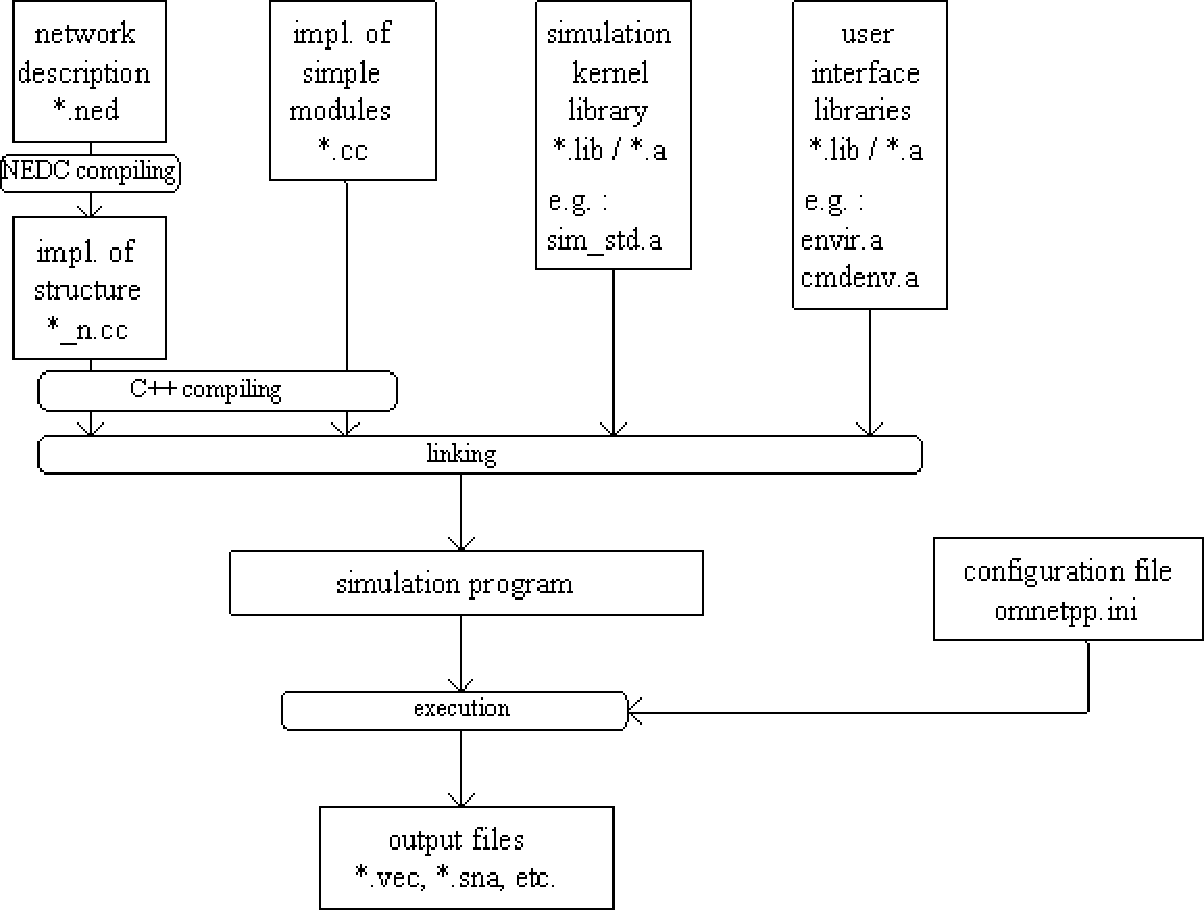
\includegraphics[width=5.992in, height=4.519in]{figures/usmanFig17}
    \caption{Building and running simulation}
  \end{center}
\end{figure}


This section discusses how to use the simulation system on the 
following platforms:
\begin{itemize}
  \item{Unix with gcc installed (and which is similar, Cygwin on Windows 
    NT)}
  \item{MSVC 6.0 on Windows NT}
  \item{Borland C++ 5.0 on Windows NT}
\end{itemize}




\section{Using Unix and gcc}

\subsection{Installation}

The installation process depends on what distribution you take 
(source, precompiled RPM, etc.) and it may change from release 
to release. The readme files in the distribution should give 
you enough (and up-to-date) guidance to go through the installation.





\subsection{Producing a makefile with the opp\_makemake script}

The \fprog{opp\_makemake} script can automatically generate the
makefile for your simulation program, based on the source files it
finds in your directory. \fprog{opp\_makemake} has several options,
the following command will display a summary:

\begin{Verbatim}
opp_makemake -h
\end{Verbatim}

To be able to use \fprog{opp\_makemake}, you have to collect all your 
sources (.ned, .cc, .h files) in one directory. (Large models 
which spread across several directories are covered later in 
this section.)


Then type 

\begin{Verbatim}
opp_makemake
\end{Verbatim}

This will create a file named Makefile\index{Makefile}. Thus if you
simply type make, your simulation program should build. The name of
the executable will be the same as the name of the directory
containing the files.


The freshly generated Makefile doesn't contain
dependencies\index{Makefile!dependencies}, it is advisable to add them
by typing \fprog[make]{make depend}. (You'll need a program named makedepend
for that, it's present on most Unix systems and in also Cygwin. The
warnings during the dependency generation process can be safely
ignored.)

In addition to the simulation executable, the makefile contains other
targets too. As mentioned, \fprog[make]{make depend} adds (or refreshes)
dependencies in the Makefile. \fprog[make]{make clean} deletes all files
that were produced by the make process. \fprog[make]{make re-makemake}
regenerates the makefile using \fprog[make]{opp\_makemake} (this is useful
if e.g.  after upgrading {\opp}, if \fprog{opp\_makemake} has
changed). \fprog[make]{make re-makemake-m} is similar to \fprog[make]{make
  re-makemake}, but it regenerates the Makefile.in file too (see
later).

If you already had a Makefile in that directory, \fprog{opp\_makemake}
will refuse overwriting it. You can force overwriting the old makefile
with the -f option:

\begin{Verbatim}
opp_makemake -f
\end{Verbatim}

If you have problems, check the path definitions (locations of include
files and libraries etc.) in the configure script\index{configure
  script} and correct them if necessary. Then re-run configure to
commit the changes to all makefiles, the \fprog{opp\_makemake} script
etc.


You can specify the user interface (Cmdenv/Tkenv) with the -u option
(with no -u, Tkenv is the default):

\begin{Verbatim}
opp_makemake -u Tkenv
\end{Verbatim}

The name of the output file\index{output!file} is set with the -o
option (the default is the name of the directory):

\begin{Verbatim}
opp_makemake -o fddi-net
\end{Verbatim}

If some of your source files are generated from other files (for
example, you use machine-generated NED files), write your make rules
into a file called makefrag. When you run \fprog{opp\_makemake}, it
will automatically insert makefrag into the resulting makefile.  With
the -i option, you can also name other files to be included into
Makefile.


If you want better portability for your models, you can generate
Makefile.in instead of Makefile with \fprog{opp\_makemake}'s -m
option. You can then use autoconf-like configure scripts to generate
the Makefile.





\subsection{Multi-directory models}

In the case of a large project, your source files may be spread across
several directories. You have to decide whether you want to use static
linking\index{static linking}, shared or run-time loaded (shared)
libraries\index{shared libraries}. Here we discuss static linking.


In each subdirectory (say trafgen/ and router/), run

\begin{Verbatim}
opp_makemake -n
\end{Verbatim}

The -n option means no linking is necessary, only compiling has 
to be done.


In your toplevel source directory, run

\begin{Verbatim}
opp_makemake trafgen/ router/
\end{Verbatim}

This results in recursive makefiles: when you build the simulation, make 
will descend into trafgen/ and router/, run make in both, then 
it will link an executable with the object files in the two directories.


You may need to use the -I option if you include files from other
directories. The -I option is for both C++ and NED
files\index{ned!include path}. In our example, you could run

\begin{Verbatim}
opp_makemake -n -I../router
\end{Verbatim}

in the trafgen/ directory and vice versa.


If you're willing to play with shared and run-time loaded libraries,
several \fprog{opp\_makemake} options and the
\texttt{[General]/load-libs=} ini file option leave you enough room to
do so.





\subsection{Static vs shared {\opp} system libraries}

Default linking uses the shared libraries\index{shared libraries}. One
reason you would want static linking is that
debugging\index{debugging} the {\opp} class library is more trouble
with shared libraries. Another reason might be that you want to run
the executable on another machine without having to worry about
setting the \fvar{LD\_LIBRARY\_PATH} variable (which should contain the name
of the directory where the {\opp} shared libraries are).

If you want static linking\index{static linking}, find the

\begin{Verbatim}
build_shared_libs=yes
\end{Verbatim}


line in the configure.user script and change it to

\begin{Verbatim}
build_shared_libs=no
\end{Verbatim}

Then you have to re-run the configure script and rebuild everything:

\begin{Verbatim}
./configure
make clean
make
\end{Verbatim}



\section{Using Win32 with MSVC}

\subsection{Prerequisite: install Tcl/Tk}

Download and install Tcl/Tk. You need at least version 8.0p1, 
but it's better to download the latest version.





\subsection{Installing {\opp}}

The installation process is not described here in detail. The 
readme files in the distribution should give you enough (and 
up-to-date) guidance to go through the installation.

What's important is that as the result of the installation, you 
should get the executables and the libraries in the bin/ and lib/ 
subdirectories within the top-level {\opp} directory.





\subsection{Building the samples from the MSVC IDE}

Unfortunately MSVC\index{MSVC} doesn't like the \texttt{.cc} extension, so first
you have to rename the \texttt{.cc} files to \texttt{.cpp}. You can do
that with samples/cc2cpp.bat.


Start the MSVC IDE and open the workspace (\texttt{.dsw}) file. Then
if you choose Build from the menu, the simulation executable should
build. If you encounter any problems, read the MSVC-related readme
file in the distribution -- it should contain more up-to-date
information than this manual.

\begin{sloppypar}
To change from Tkenv to Cmdenv or vica versa, choose Build{\textbar}Set 
active configuration from the menu and select one of 'Debug-Tkenv', 
'Release-Tkenv', 'Debug-Cmdenv', 'Release-Cmdenv', then re-link 
the executable.
\end{sloppypar}

If you have big models, you'll probably have to increase the stack
size. You'll find the setting under Project{\textbar}Settings
--\texttt{>} 'Link' tab --\texttt{>} choose 'Output' from combo
--\texttt{>} Stack allocations, Reserve. Be aware that if you don't
specify anything here, MSVC defaults to 1MB -- way too small.\\
If you need to modify the names of the Tcl/Tk libs (because you
installed a Tcl/Tk version other than 8.2), see
Project{\textbar}Settings --\texttt{>} 'Link' tab --\texttt{>} choose
'Input' from combo --\texttt{>} Libraries.

The Tcl/Tk install program normally sets the \fvar{TCL\_LIBRARY}
environment variable needed by Tcl applications. However, if you see
the ''can't find a usable init.tcl...'' error message when you start a
simulation program (or Gned or Plove), then that didn't happen and you
have to set the variable yourself.




\subsection{Creating project files for your simulations}

\begin{enumerate}
\item{Start by copying \& renaming one of the \texttt{.dsp} files from
    the samples directory. It already contains the Tkenv/Cmdenv
    configurations, etc.}
\item{ Rename all \texttt{.cc} files to \texttt{.cpp} (\texttt{ren
      *.cc *.cpp}) and add them to the project.}
\item{Add the \texttt{.ned} files to the project and set custom build
    option for them:

\begin{Verbatim}
Description: NED Compiling $(InputPath) 
Command: nedc -s _n.cpp $(InputPath)
Outputs: $(InputPath)_n.cpp
\end{Verbatim}
%% $


\textit{Hint: you can select all \texttt{.ned} files together, and
  'All configurations' from the combo at the left of the Settings
  dialog, and then you have to type this settings only once.}}


\item{For each \texttt{.ned} file, add a corresponding
    \texttt{\_n.cpp} file.
    
    \textit{Hint: if you compile the \texttt{.ned} files (choose
      'Compile' from the menu), the} \texttt{\_n.cpp} \textit{files will be
      created, and you can select them all at once in the 'Add files'
      dialog.}}
\item{Make sure to turn off exception handling\index{exception
      handling} and RTTI\index{RTTI} (they interfere with the
    coroutine library), and set the necessary reserved stack size.}
\item{Note: for Tkenv, link with \texttt{sim\_std.lib},
    \texttt{envir.lib}, \texttt{tkenv.lib} and the Tcl/Tk libraries
    (link as Win32 Console app...). For Cmdenv, you need to link with \texttt{sim\_std.lib}, \texttt{envir.lib}, and \texttt{cmdenv.lib}.\\
    It is planned to create wizards in the future to ease some of
    these steps.}
\end{enumerate}




\subsection{Using Plove}

If you want to use Plove\index{Plove}, you should download and install
Gnuplot\index{Gnuplot}.  You'll also need a couple of Unix tools like
\fprog{grep} and \fprog{awk}, the easiest way to get them is to
download and install the Cygwin package from
\href{http://www.cygnus.com}{www.cygnus.com}.  When you have
everything installed, start Plove and set the appropriate
configuration in Options{\textbar}External programs. If you entered
everything correctly, Plove should work.


A usual caveat is that Gnuplot expects forward slashes in filenames
and Plove supplies backslashes or vica versa (there are multiple
incompatible builds of Gnuplot on NT); if you suspect this might be
the problem, reverse the slash/backslash setting in
Options{\textbar}External programs.





\section{Hints for using Borland C++ and other compilers}

\subsection{Building {\opp}}

{\opp} currently doesn't support the Borland C++\index{Borland C++}.
This doesn't mean that the sources won't build (most probably they
will), but I am unable to maintain the respective makefiles.


However, the next sections contain some hints how to build simulation 
programs once you got the libraries compiled.





\subsection{Setting up a project file}

What you will need to have in your project file:
\begin{itemize}
  \item{your simple module C++ sources;}
  \item{your NED files\index{ned!files};}
  \item{for each NED file, the C++ file it will compile into (the
      \texttt{\_n.cc} file). Place the \texttt{.ned} file under the
      \texttt{\_n.cc} file in the project tree hierarchy.}
  \item{the {\opp} libraries: \texttt{sim\_std.lib},
      \texttt{envir.lib}, plus \texttt{cmdenv.lib} or
      \texttt{tkenv.lib}, depending on which user interface you want
      to link in. You also need the Tcl and Tk libraries if you're
      using Tkenv.}
\end{itemize}


The project options have to be set up like this:
\begin{itemize}
\item{Compile as a 32-bit flat console application. None of the
    special libraries (OWL, MFC, Class Library, OCF etc) are needed.}
\item{You have to turn off exception handling\index{exception
      handling}, it conflicts with the coroutine
    library\index{coroutine library} somehow. In the IDE:
    Options{\textbar}Project --\texttt{>} C++ Options --\texttt{>}
    Exception Handling/RTTI --\texttt{>} clear [ ] Enable exceptions.
    It must be done both when compiling the libraries and when
    compiling simulation applications.}
\item{Borland C++ does not recognize the \texttt{.cc} extension as
    C++. You have to teach it: Options{\textbar}Tools --\texttt{>}
    select CppCompile --\texttt{>} Edit --\texttt{>} Advanced
    --\texttt{>} add the \texttt{.cc} extension to the Translate From
    and Default For entries. Do the same with the EditText tool.}
\item{You also have to teach Borland C++ how to handle \texttt{.ned}
    files.  Select Options{\textbar}Tools --\texttt{>} New. Fill in
    the dialog as follows:
\begin{Verbatim}
  Name: NEDCompile

  Path: ..\..\src\nedc\nedc.exe

  Command Line: $NOSWAP $CAP MSG(BORL2MSG) $EDNAME

  Menu Text: NED Compile

  Help Hint: OMNeT++ NED compiler
\end{Verbatim}
%%$
  Select Advanced, and fill in the dialog:
\begin{Verbatim}
  Type: Translator
  Translate From:.ned
  Translate To:.cc
  Default For:.ned
  
\end{Verbatim}
}

\sloppy
\item{If you're going to build a LARGE model, be sure to
  increase the stack size\index{stack!size} in
  Options{\textbar}Project options{\textbar}Linker{\textbar}32-bit
  Linker{\textbar}Reserved stack size. The default is 0x1000000 (1MB),
  which is hardly enough for {\opp} simulations. Increase it to 64MB
  for example: 0x40000000. If the simulation exceeds the stack size
  configured here, you'll get nice exceptions, General Protection
  Faults and the like.}
\end{itemize}


%%% Local Variables: 
%%% mode: latex
%%% TeX-master: "usman"
%%% End: 
